% !TeX program = pdflatex
%==============================================================================
%  Aula 01 --- Introdução ao Aprendizado de Máquina
%  VERSÃO DO ALUNO: texto para leitura autônoma, fora da sala.
%  (O roteiro de sala correspondente é "01 Introducao.tex".)
%==============================================================================
\documentclass[11pt,a4paper]{article}
\usepackage[aluno]{../../recursos/latex/estilo-notas}

\title{}
\date{}

\begin{document}
\cabecalhoaula{01}{Introdução ao Aprendizado de Máquina}{AME cap.~1; ISLP cap.~1--2}

%==============================================================================
\section*{O que você vai aprender}
%==============================================================================
Ao final desta aula você deve ser capaz de:
\begin{itemize}[leftmargin=1.4cm]
  \item enunciar o problema de aprendizado supervisionado e distinguir
        \emph{regressão} de \emph{classificação};
  \item escrever a função de regressão $r(\x)=\E[Y\mid\X=\x]$ e justificá-la como
        solução do problema de predição sob perda quadrática;
  \item diferenciar os objetivos de \emph{predição} e de \emph{inferência} e
        relacionar isso às ``duas culturas'' da modelagem estatística;
  \item definir \emph{risco} e \emph{risco empírico} e explicar por que minimizar o
        risco empírico no treino não basta;
  \item explicar \emph{super} e \emph{subajuste} e a decomposição
        \emph{viés--variância};
  \item identificar o papel dos \emph{tuning parameters} no controle da
        complexidade.
\end{itemize}

\noindent
Esta é a aula que fixa a \textbf{linguagem} de todo o curso, então vale ir devagar
na notação: tudo o que vier depois --- regressão linear, KNN, árvores, SVM,
classificação --- é caso particular do arcabouço montado aqui. Comece pela pergunta
que a aula inteira responde:

\begin{center}\itshape
  o que significa, exatamente, dizer que um modelo ``aprendeu''?
\end{center}

\noindent
Guarde o seu palpite. Na Seção~\ref{sec:risco} teremos uma definição precisa, e ela
provavelmente não vai coincidir com a intuição de ``acertar os dados que eu já
tenho''.

%==============================================================================
\section{O que é aprendizado de máquina?}
%==============================================================================
Aprendizado de máquina (AM) nasceu nos anos 1960 como ramo da inteligência
artificial voltado a \emph{aprender padrões a partir de dados}. A partir do final
dos anos 1990 a área se consolidou e passou a ter forte interseção com a
estatística. Neste curso adotamos a \textbf{ótica estatística} do [AME]: tratamos
os dados como realizações de variáveis aleatórias e usamos probabilidade e
inferência para entender \emph{quando} e \emph{por que} um método funciona.

Trabalhamos em três grandes cenários:
\begin{description}[leftmargin=2.6cm,style=nextline]
  \item[Supervisionado] observamos pares $(\x,y)$ (covariáveis e rótulo) e
        queremos prever $y$ a partir de $\x$. Subdivide-se em \emph{regressão}
        ($Y$ quantitativo) e \emph{classificação} ($Y$ qualitativo).
  \item[Não supervisionado] observamos apenas $\x$ (sem rótulos) e buscamos
        estrutura: agrupamento, redução de dimensionalidade, associação.
  \item[Por reforço] um agente aprende por tentativa e erro interagindo com um
        ambiente (fora do escopo deste curso).
\end{description}
A maior parte do curso é sobre aprendizado supervisionado; o aprendizado não
supervisionado aparece nas aulas extras ($k$-médias, PCA).

\begin{atencao}[um erro de tradução que confunde muita gente]
$Y$ \emph{quantitativa} $\Rightarrow$ problema de \textbf{regressão}.
$Y$ \emph{qualitativa} $\Rightarrow$ problema de \textbf{classificação}.
Na dúvida, pergunte se faz sentido calcular a \emph{média} da resposta: faz sentido
falar em ``temperatura média'' (regressão), não faz sentido em ``e-mail médio entre
spam e não-spam'' (classificação).
\end{atencao}

%==============================================================================
\section{Notação e suposições}
%==============================================================================
Seja $Y\in\R$ a \textbf{variável resposta} (também: variável dependente, rótulo,
\emph{label}) e $\x=(x_1,\dots,x_d)\in\R^d$ o vetor de \textbf{covariáveis}
(também: atributos, preditores, \emph{features}, variáveis explicativas). O
objetivo central da Parte~I do [AME] é estimar a \textbf{função de regressão}
\begin{equation}\label{eq:r}
  r(\x) \;:=\; \E[Y\mid \X=\x].
\end{equation}
Quando $Y$ é quantitativo, temos um problema de \textbf{regressão}; quando $Y$ é
qualitativo, um problema de \textbf{classificação}.

\begin{definicao}[Amostra de treino]
Salvo menção em contrário, supomos uma amostra i.i.d.
$\Dados=\{(\X_1,Y_1),\dots,(\X_n,Y_n)\}$, com $(\X_i,Y_i)\sim (\X,Y)$, de uma
distribuição conjunta $P$ desconhecida. Denotamos por $x_{i,j}$ o valor da
$j$-ésima covariável na $i$-ésima observação, $\X_i=(x_{i,1},\dots,x_{i,d})$.
\end{definicao}

\noindent
Vale a pena visualizar os dados como uma tabela, que é literalmente o formato em que
eles chegam num arquivo \texttt{.csv}: cada \emph{linha} é uma observação, cada
\emph{coluna} é uma covariável, e a última coluna é a resposta.
\begin{center}\small
\renewcommand{\arraystretch}{1.25}
\begin{tabular}{@{}c c c c c@{}}
\toprule
\textbf{Resposta} & \multicolumn{4}{c}{\textbf{Covariáveis}} \\
\midrule
$Y_1$    & $x_{1,1}$ & $x_{1,2}$ & $\cdots$ & $x_{1,d}$ \\
$\vdots$ & $\vdots$  & $\vdots$  &          & $\vdots$  \\
$Y_n$    & $x_{n,1}$ & $x_{n,2}$ & $\cdots$ & $x_{n,d}$ \\
\bottomrule
\end{tabular}
\end{center}
Aqui $n$ é o \emph{número de observações} e $d$ o \emph{número de covariáveis}.
Boa parte das dificuldades do curso aparece quando $d$ cresce em relação a $n$ ---
uma tabela mais larga do que alta. Voltaremos a isso já na Aula~02.

\begin{atencao}
A suposição i.i.d.\ é forte e nem sempre razoável (séries temporais, dados
espaciais, viés de seleção, \emph{dataset shift}). Voltaremos a isso na Aula~09;
por ora ela é o nosso ``mundo ideal''. A distribuição $P$ é \emph{fixa} mas
\emph{desconhecida}: é a fonte de toda a incerteza.
\end{atencao}

%==============================================================================
\section{Por que estimar a função de regressão? Predição versus inferência}
%==============================================================================
Há duas razões distintas para estimar $r$:
\begin{itemize}[leftmargin=1.4cm]
  \item \textbf{Predição.} Queremos um bom palpite $\rhat(\x)$ para o $Y$ de uma
        nova observação com covariáveis $\x$. Aqui $\rhat$ pode ser uma
        ``caixa-preta'': interessa o \emph{acerto}, não a forma.
  \item \textbf{Inferência.} Queremos \emph{entender} a relação entre $\X$ e $Y$:
        quais covariáveis importam, qual o sinal e a magnitude do efeito, há
        interações? Aqui interessa a \emph{interpretabilidade} do modelo.
\end{itemize}

\noindent
Quatro exemplos do [AME] deixam a diferença concreta:

\begin{exemplo}[Expectativa de vida e PIB per capita]
Para 211 países, $Y$ é a expectativa de vida e $x$ o PIB per capita. Estimar
$\E[Y\mid x]$ serve tanto para \emph{predizer} a expectativa de vida de um país cujo
PIB conhecemos quanto para \emph{testar} se existe relação entre as duas variáveis.
Objetivo misto.
\end{exemplo}

\begin{exemplo}[Distância de uma galáxia até a Terra]
O \emph{redshift} de uma galáxia mede sua distância. A espectroscopia o determina
com precisão, mas é cara e lenta. A alternativa é estimar $r(\x)$ tomando $\X_i$ como
a \emph{imagem} da $i$-ésima galáxia. Aqui a relação entre cada pixel e a resposta não
interessa a ninguém: objetivo puramente \textbf{preditivo}.
\end{exemplo}

\begin{exemplo}[Direção do olhar a partir de uma foto]
No \emph{Isomap face data}, $Y$ é a direção para a qual a pessoa olha e $\x$ é a
imagem do rosto. De novo, puramente preditivo.
\end{exemplo}

\begin{exemplo}[Ano de lançamento de músicas]
No \emph{YearPredictionMSD}, $\x$ traz timbre, ``energia'', ``dançabilidade'' etc.\ e
$Y$ é o ano de lançamento. Queremos (i) predizer o ano e (ii) entender como o perfil
das músicas mudou --- por exemplo, os anos 70 eram mais dançáveis? Objetivo misto.
\end{exemplo}

\begin{ideia}
Por que $r(\x)=\E[Y\mid\X=\x]$ é o alvo ``certo'' para predição? Porque, sob a
perda quadrática, a função que minimiza o erro esperado de predição é exatamente a
esperança condicional.
\end{ideia}

\begin{proposicao}[$r$ minimiza o erro quadrático esperado]\label{prop:r}
Entre todas as funções $g:\R^d\to\R$, a função de regressão
$r(\x)=\E[Y\mid\X=\x]$ minimiza o erro quadrático esperado
$\E\big[(Y-g(\X))^2\big]$.
\end{proposicao}
\begin{proof}
Fixe $\x$ e escreva $\E[(Y-g(\X))^2\mid\X=\x]$. Somando e subtraindo $r(\x)$,
\[
  \E\big[(Y-g(\x))^2\mid\X=\x\big]
  = \E\big[(Y-r(\x))^2\mid\X=\x\big] + \big(r(\x)-g(\x)\big)^2,
\]
pois o termo cruzado se anula:
$\E[(Y-r(\x))(r(\x)-g(\x))\mid\X=\x]=(r(\x)-g(\x))\,\E[Y-r(\x)\mid\X=\x]=0$.
O primeiro termo não depende de $g$ e o segundo é minimizado (zerado) por
$g(\x)=r(\x)$. Tomando esperança sobre $\X$, segue o resultado.
\end{proof}

\noindent
Vale destrinchar o passo que faz a conta funcionar, porque ele reaparece o curso
inteiro. O termo cruzado se anula porque, \emph{dado} $\X=\x$, a quantidade
$r(\x)-g(\x)$ é uma \textbf{constante} --- ela sai da esperança --- e o que sobra é
$\E[Y-r(\x)\mid\X=\x]=\E[Y\mid\X=\x]-r(\x)=0$, pela própria definição
\eqref{eq:r} de $r$. Em palavras: \emph{o erro que resta depois de acertar a média
condicional não tem correlação com nada que dependa só de $\x$}. É a mesma ideia de
uma projeção ortogonal.

\begin{observacao}
A decomposição acima já contém a semente do \emph{erro irredutível}: mesmo
conhecendo $r$ perfeitamente, resta $\E[(Y-r(\X))^2]=\E[\Var(Y\mid\X)]>0$ em
geral, pois $Y$ não é função determinística de $\X$.
\end{observacao}

\subsection{As duas culturas}
Leo Breiman (2001) descreveu duas posturas de modelagem:
\begin{itemize}[leftmargin=1.4cm]
  \item \textbf{Cultura dos modelos de dados:} supõe-se um modelo estocástico
        (por exemplo, linear gaussiano) e o foco é estimar e interpretar seus
        parâmetros. Testar as suposições (normalidade, linearidade,
        homocedasticidade) é parte central do trabalho. Tradição estatística
        clássica.
  \item \textbf{Cultura dos modelos algorítmicos:} trata-se o mecanismo gerador
        como desconhecido e busca-se uma função preditora com bom desempenho
        (florestas, \emph{boosting}, redes). Muitas vezes não há modelo
        probabilístico explícito por trás. Tradição de AM.
\end{itemize}
O [AME] --- e este curso --- fica majoritariamente na segunda: buscamos estimar
$r(\x)$ \emph{sem supor} que nossos modelos contêm a verdadeira função de regressão.
Mas usamos a teoria estatística da primeira para \emph{avaliar} os métodos da
segunda.

Um exemplo ajuda a sentir a diferença de objetivo. Comparar a previsão de demanda de
energia (predição pura: ninguém precisa entender o modelo, só acertar o número) com
a avaliação do efeito de um medicamento (inferência: o número sozinho não serve, é
preciso saber \emph{o quanto} e \emph{por quê}). Pergunte-se: em qual desses um
modelo caixa-preta altamente preciso seria \emph{inaceitável}? A resposta explica por
que interpretabilidade é um requisito, e não um capricho, em várias áreas.

%==============================================================================
\section{A função de risco}\label{sec:risco}
%==============================================================================
Para comparar candidatos a preditor precisamos de um critério de qualidade. Dado
uma \textbf{função de perda} $L(y,\hat y)\ge 0$, definimos o risco.

\begin{definicao}[Risco]
O \textbf{risco} (ou erro de generalização) de uma função $g$ é
\begin{equation}\label{eq:risco}
  \risco(g) \;=\; \E\big[L(Y,g(\X))\big],
\end{equation}
a perda esperada sobre uma observação \emph{nova} $(\X,Y)\sim P$.
\end{definicao}

Em regressão usamos tipicamente a perda quadrática $L(y,\hat y)=(y-\hat y)^2$, e
então $\risco(g)=\E[(Y-g(\X))^2]$. Pela Proposição~\ref{prop:r}, $r$ é o
\emph{minimizador} do risco. A decomposição fundamental do risco de $g$ é
\begin{equation}\label{eq:decomprisco}
  \risco(g) \;=\; \underbrace{\E\big[(g(\X)-r(\X))^2\big]}_{\text{excesso de risco}}
              \;+\; \underbrace{\E\big[\Var(Y\mid\X)\big]}_{\text{erro irredutível}},
\end{equation}
que é exatamente a conta da Proposição~\ref{prop:r} escrita de outro jeito
(Teorema~1 do [AME]). A leitura é: \emph{o risco de $g$ se parte na distância entre
$g$ e o alvo $r$, que depende de você, mais um piso que não depende de ninguém}.

\begin{atencao}
Aqui está a resposta à pergunta da abertura. Um modelo \textbf{não} ``aprendeu''
quando acerta os dados que já viu --- ele aprendeu quando tem \textbf{risco baixo},
e risco é uma esperança sobre observações \emph{que ele nunca viu}. Toda a
dificuldade do curso vem daí: $P$ é desconhecida, então $\risco(g)$ é uma quantidade
\emph{teórica} que precisamos \emph{estimar}. É o tema da Aula~03.
\end{atencao}

\subsection{Risco empírico}
O estimador natural do risco, dado um conjunto de dados $\{(\X_i,Y_i)\}$, é a média
das perdas:
\begin{equation}\label{eq:remp}
  \riscohat(g) \;=\; \frac1n \sum_{i=1}^n L\big(Y_i,g(\X_i)\big).
\end{equation}
Se calculado \emph{nos mesmos dados usados para treinar} $g$, ele subestima
sistematicamente o risco --- daí a necessidade de dados de teste/validação. A razão é
simples quando dita em voz alta: $g$ foi \emph{escolhida} para ir bem justamente
naqueles pontos. Medir o desempenho ali é como corrigir a prova com o gabarito que o
próprio aluno escreveu.

Se, em vez disso, $\riscohat$ for calculado num conjunto de \textbf{teste} de tamanho
$m$ que não participou de nada, ele é uma média de $m$ variáveis i.i.d.\ e o Teorema
Central do Limite dá até uma barra de erro:
\begin{equation}\label{eq:ic}
  \riscohat(g) \;\pm\; 2\sqrt{\widehat\sigma^2/m},
  \qquad
  \widehat\sigma^2=\frac1m\sum_{k=1}^m (W_k-\overline W)^2,
  \quad W_k=\big(Y_k-g(\X_k)\big)^2,
\end{equation}
um intervalo de confiança aproximado de 95\% para $\risco(g)$. Isso é mais útil do
que parece: dois modelos cujos intervalos se sobrepõem largamente \emph{não} foram
distinguidos pelo seu conjunto de teste, por mais que um deles tenha ficado com o
número menor. E note a consequência de projeto: como o erro do intervalo cai com
$\sqrt m$, estimar o risco é uma tarefa muito mais barata do que construir um bom
preditor --- com $n$ grande, dá para reservar bem menos que 30\% para teste.

\begin{observacao}[Risco condicional e risco esperado]
Há uma sutileza na Equação~\eqref{eq:risco}. Se $g$ é tratada como \emph{fixa}, a
esperança é só sobre a nova observação $(\X,Y)$ e temos o \textbf{risco condicional}:
uma garantia sobre \emph{aquela} função. Se tratamos $g=\ghat$ como aleatória (ela é
função dos dados de treino), a esperança também percorre todas as amostras
possíveis e temos o \textbf{risco esperado}: uma garantia sobre o \emph{procedimento}
que gerou $\ghat$, não sobre o resultado de uma rodada específica. Usaremos os dois
conforme o contexto; a decomposição viés--variância da
Seção~\ref{sec:viesvariancia}, por exemplo, é sobre o risco esperado.
\end{observacao}

%==============================================================================
\section{Seleção de modelos: super e subajuste}
%==============================================================================
Um método de AM em geral define uma \textbf{classe de funções} $\Hcal$ (a
``flexibilidade'' do modelo) e escolhe dentro dela aquela que melhor ajusta os
dados. Há uma tensão:
\begin{itemize}[leftmargin=1.4cm]
  \item \textbf{Subajuste (\emph{underfitting}):} $\Hcal$ é simples demais para
        capturar $r$. Erro de treino \emph{e} de teste altos. Modelo
        ``enviesado''.
  \item \textbf{Superajuste (\emph{overfitting}):} $\Hcal$ é flexível demais e
        ajusta o ruído da amostra. Erro de treino baixo, erro de teste alto.
        Modelo ``variável''.
\end{itemize}

Para ver isso acontecer, vamos fabricar um problema em que a resposta é conhecida.
Tome $X\sim\mathrm{Unif}(-3,3)$ e
\begin{equation}\label{eq:pop}
  Y = \underbrace{\operatorname{sen}(1{,}5X)+0{,}3X}_{r(x)} + \varepsilon,
  \qquad \varepsilon\sim N(0,\sigma^2),\quad \sigma=0{,}7 .
\end{equation}
Como \emph{nós} inventamos a população, sabemos que $r$ é aquela e que o erro
irredutível vale $\sigma^2=0{,}49$. Sorteamos $n=50$ pontos de treino e ajustamos
polinômios de graus crescentes. A Figura~\ref{fig:ajustes} mostra três deles.

\begin{figure}[htbp]
  \centering
  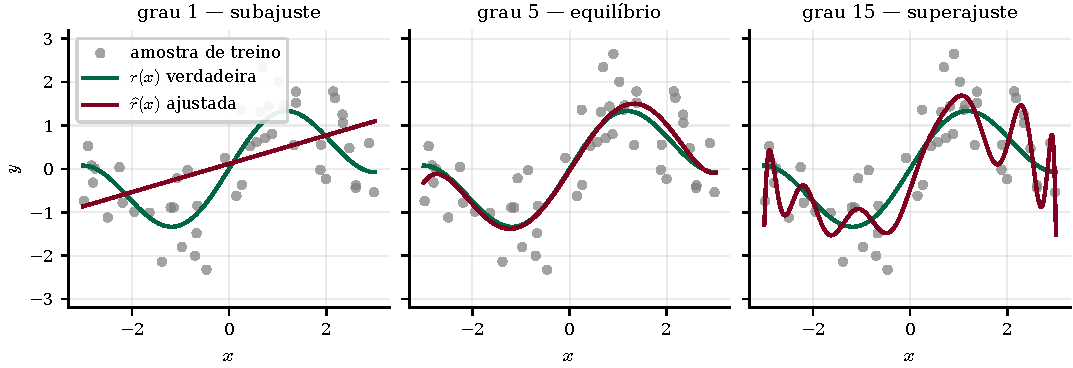
\includegraphics[width=\textwidth]{../../recursos/figuras/01-ajustes.pdf}
  \caption{Três ajustes sobre \emph{a mesma} amostra de $n=50$ pontos. O grau~1 é
  rígido demais para acompanhar a curvatura de $r$ (subajuste). O grau~15 passa perto
  de quase todos os pontos, inclusive perseguindo o ruído, e oscila onde $r$ é suave
  (superajuste). O grau~5 acerta o essencial.}
  \label{fig:ajustes}
\end{figure}

Repetindo isso para cada grau e medindo os dois erros, obtemos o comportamento
típico: o erro de treino cai monotonicamente, mas o risco tem forma de ``U'' ---
existe um ponto de complexidade ótima (Figura~\ref{fig:curvaU}).

\begin{figure}[htbp]
  \centering
  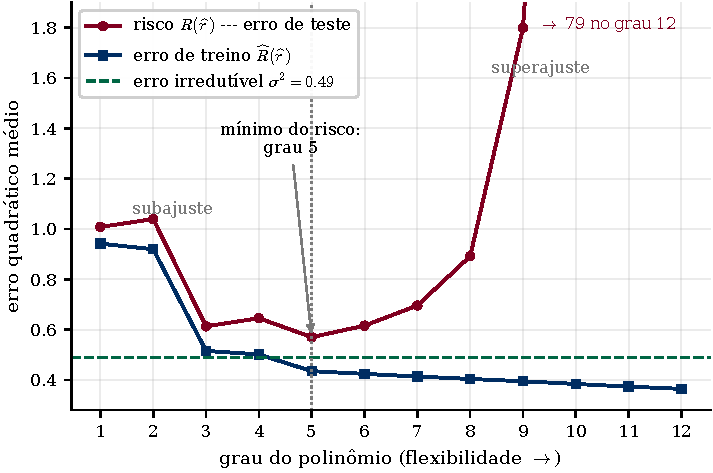
\includegraphics[width=0.72\textwidth]{../../recursos/figuras/01-curva-U.pdf}
  \caption{Erro de treino e risco em função do grau, médias sobre 400 amostras de
  treino da população \eqref{eq:pop}. O erro de treino cai sempre e chega a
  \emph{furar} o piso $\sigma^2$ --- sinal inequívoco de que está medindo ruído, não
  sinal. O risco desce, atinge o mínimo no grau~5 e volta a subir; no grau~12 já vale
  $79$, mais de 160 vezes o mínimo.}
  \label{fig:curvaU}
\end{figure}

Duas leituras que valem mais do que parecem à primeira vista:

\begin{itemize}[leftmargin=1.4cm]
  \item \textbf{O erro de treino fura o $\sigma^2$.} A partir do grau~3 ele fica
        abaixo de $0{,}49$, que é o menor risco alcançável por \emph{qualquer}
        função. Nenhum preditor pode ser tão bom assim; o que ele está fazendo é
        ajustar o ruído daquela amostra específica.
  \item \textbf{O risco nunca desce abaixo de $\sigma^2$.} A linha tracejada é um
        piso intransponível. Se o seu erro de teste chegar perto dele, você está no
        limite do problema, não do método --- procurar um modelo melhor é perda de
        tempo.
\end{itemize}

\begin{atencao}[o que ``superajuste'' quer dizer, exatamente]
O [ISLP] é preciso aqui, e a precisão importa: superajuste é o caso em que
\textbf{um modelo menos flexível teria dado um risco menor}. Não é sinônimo de ``erro
de treino menor que o de teste'' --- isso acontece quase sempre, com ou sem
superajuste, porque quase todo método minimiza direta ou indiretamente o erro de
treino.
\end{atencao}

O quanto o ``U'' é profundo depende de quão longe $r$ está da classe de modelos que
você usa. Se $r$ for quase linear, o mínimo aparece cedo e o lado direito sobe rápido;
se $r$ for muito não linear, o erro despenca bastante antes de voltar a subir. A forma
geral, porém, é sempre a mesma.

\subsection{Um exemplo que contraria a intuição}
Poderia parecer que, sabendo a forma correta do modelo, o melhor a fazer é ajustá-la.
Não é bem assim, e o [AME] traz um exemplo simulado que convém guardar. Gere dados com
\[
  Y\mid \x \sim N(\bbeta^\top\x,\,1),\qquad
  \bbeta=(0,\;3,\;2,\;0{,}2,\;0{,}1,\;0{,}1),\qquad
  \x=(1,x,x^2,\dots,x^5),
\]
ou seja, a regressão verdadeira \emph{é} um polinômio de grau~5. Ajuste dois modelos:
um polinômio de grau~5 (especificação correta) e um de grau~2 (incorreta). Repetindo
o experimento para 1000 conjuntos de treino, o modelo de \textbf{grau~2} teve risco
esperado menor --- e ganhou do modelo correto em \textbf{97,8\%} das amostras.

\begin{ideia}
Especificar o modelo corretamente \textbf{não} garante melhor poder preditivo. Os
três últimos coeficientes de $\bbeta$ são minúsculos ($0{,}2$, $0{,}1$, $0{,}1$): o
ganho de viés ao incluí-los é desprezível perto do custo de \emph{estimá-los}. O
modelo errado, porém mais simples, tem variância bem menor e sai na frente.
\end{ideia}

\noindent
Essa é a diferença de mentalidade entre a estatística inferencial clássica --- em que
se busca um estimador não viesado --- e a inferência preditiva, em que se aceita viés
de bom grado desde que a variância caia mais do que o viés sobe.

\begin{observacao}
Uma ressalva honesta: interpolar os dados não implica necessariamente superajustar.
Redes neurais muito grandes frequentemente interpolam o treino e ainda assim
generalizam bem, um fenômeno conhecido como \emph{descida dupla} (Belkin et al.,
2019). A curva em ``U'' é a regra para os métodos deste curso, não uma lei da
natureza.
\end{observacao}

\subsection{O balanço entre viés e variância}\label{sec:viesvariancia}
Considere um estimador $\rhat$ construído a partir da amostra aleatória $\Dados$.
Em um ponto fixo $\x_0$, sob perda quadrática, vale a decomposição clássica:
\begin{equation}\label{eq:bv}
  \E_{\Dados}\!\big[(Y_0-\rhat(\x_0))^2\big]
  = \underbrace{\big(\E_{\Dados}[\rhat(\x_0)]-r(\x_0)\big)^2}_{\text{viés}^2}
  + \underbrace{\Var_{\Dados}\!\big(\rhat(\x_0)\big)}_{\text{variância}}
  + \underbrace{\sigma^2(\x_0)}_{\text{irredutível}},
\end{equation}
onde $Y_0$ é uma resposta nova em $\x_0$ e $\sigma^2(\x_0)=\Var(Y\mid\X=\x_0)$.

\begin{teorema}[Decomposição viés--variância]\label{teo:bv}
Vale a identidade \eqref{eq:bv}.
\end{teorema}
\begin{proof}
Escreva $Y_0-\rhat(\x_0) = \big(Y_0-r(\x_0)\big) + \big(r(\x_0)-\rhat(\x_0)\big)$.
O primeiro parêntese tem média zero e variância $\sigma^2(\x_0)$ e é independente
de $\Dados$. Para o segundo, some e subtraia $\E_{\Dados}[\rhat(\x_0)]$ e
expanda o quadrado; o termo cruzado se anula porque
$\E_{\Dados}[\rhat(\x_0)-\E_{\Dados}\rhat(\x_0)]=0$. Reagrupando os três quadrados
obtém-se \eqref{eq:bv}.
\end{proof}

\noindent
Cada termo tem um significado que vale nomear:
\begin{description}[leftmargin=2.4cm,style=nextline]
  \item[Viés] o erro que você comete por aproximar um problema complicado com um
        modelo mais simples. Uma reta ajustada a uma senoide erra \emph{em média},
        por mais dados que você colete.
  \item[Variância] o quanto $\rhat$ mudaria se você tivesse sorteado \emph{outra}
        amostra de treino do mesmo tamanho. Um polinômio de grau 15 sobre 50 pontos
        muda radicalmente de uma amostra para a outra; uma reta quase não muda.
  \item[Irredutível] o ruído de $Y$ em torno de $r$. Não depende do que você faça.
\end{description}

A Figura~\ref{fig:bv} mede os três termos na população \eqref{eq:pop} e confirma a
identidade numericamente.

\begin{figure}[htbp]
  \centering
  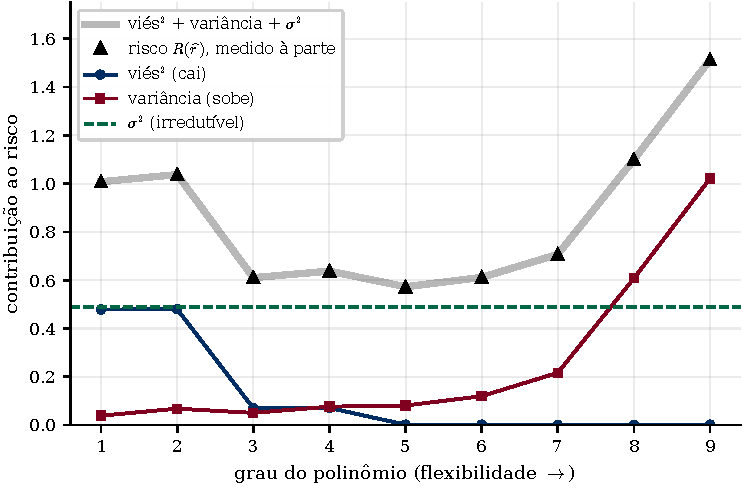
\includegraphics[width=0.78\textwidth]{../../recursos/figuras/01-vies-variancia.pdf}
  \caption{Os três termos de \eqref{eq:bv} em função do grau, sobre 500 amostras de
  treino. O viés$^2$ desaba (do grau~5 em diante o polinômio já reproduz $r$); a
  variância sobe sem parar; $\sigma^2$ é constante. A faixa cinza é a \emph{soma} dos
  três, e os triângulos pretos são o risco medido \emph{à parte}, sem usar a
  decomposição: eles caem exatamente sobre a faixa. A identidade fecha com folga
  máxima de $2\times10^{-16}$, ou seja, na precisão da máquina.}
  \label{fig:bv}
\end{figure}

\begin{ideia}
Modelos \emph{flexíveis} têm baixo viés e alta variância; modelos \emph{rígidos}
têm alto viés e baixa variância. Selecionar um modelo é, em essência,
\textbf{escolher o ponto do balanço viés--variância} que minimiza o risco. Não dá
para zerar os dois ao mesmo tempo com $n$ finito.
\end{ideia}

\noindent
E por que o mínimo existe? Porque as duas curvas não mudam no mesmo ritmo: no começo,
aumentar a flexibilidade derruba o viés \emph{mais rápido} do que levanta a variância,
e o risco cai. A partir de certo ponto o viés já está perto de zero e não há mais nada
a ganhar, mas a variância continua subindo --- e o risco volta a crescer. O ``U'' da
Figura~\ref{fig:curvaU} é a soma dessas duas corridas em ritmos diferentes.

\begin{atencao}
Na Figura~\ref{fig:bv} pudemos calcular viés e variância porque \emph{inventamos} a
população e conhecemos $r$. Num problema real isso é impossível: $r$ é justamente o
que não sabemos. A decomposição é uma ferramenta de \emph{raciocínio} --- serve para
você prever em que direção mexer --- e não um diagnóstico que se roda nos dados.
\end{atencao}

%==============================================================================
\section{Tuning parameters}
%==============================================================================
A flexibilidade de um método costuma ser controlada por um ou mais
\textbf{hiperparâmetros} (\emph{tuning parameters}), que \emph{não} são estimados
junto com o ajuste, mas escolhidos ``por fora''. No exemplo desta aula, o
hiperparâmetro é o grau do polinômio, e a Figura~\ref{fig:curvaU} é literalmente o
gráfico do risco em função dele. Exemplos que veremos:
\begin{center}\small
\renewcommand{\arraystretch}{1.25}
\begin{tabular}{@{}lll@{}}
\toprule
\textbf{Método} & \textbf{Hiperparâmetro} & \textbf{Efeito de aumentá-lo} \\
\midrule
Regressão polinomial & grau do polinômio & mais flexível ($\uparrow$ variância) \\
Lasso / Ridge        & $\lambda$ (penalização) & mais rígido ($\uparrow$ viés) \\
$k$ vizinhos (KNN)   & $k$ & mais rígido ($\uparrow$ viés) \\
Árvore               & profundidade / $\alpha$ de poda & (depende do parâmetro) \\
\bottomrule
\end{tabular}
\end{center}
A escolha desses parâmetros é um problema de \emph{seleção de modelos}, resolvido
estimando o risco para vários valores e tomando o melhor --- tema central da
Aula~03.

\begin{atencao}
Hiperparâmetros devem ser escolhidos \emph{sem olhar o conjunto de teste}. Usar o
teste para escolher $\lambda$ ou $k$ e depois reportar o erro nesse mesmo teste é
uma forma de vazamento de dados (\emph{data leakage}) que infla o desempenho. A
divisão em \emph{três} partes --- treino, validação e teste --- existe exatamente
para isso: o treino ajusta, a validação escolhe o hiperparâmetro, e o teste, tocado
uma única vez no fim, estima o risco do vencedor.
\end{atencao}

\subsection*{Uma alternativa: penalização}
Nem sempre é preciso separar dados para estimar o risco. Como o erro de treino
subestima o risco tanto mais quanto mais parâmetros o modelo tem, pode-se
\emph{corrigi-lo} somando uma medida de complexidade:
\[
  \risco(g) \;\approx\; \mathrm{EQM}(g) + P(g),
  \qquad
  P(g)=\frac{2p\,\widehat\sigma^2}{n} \ \ (\text{AIC}),
  \qquad
  P(g)=\frac{\log(n)\,p\,\widehat\sigma^2}{n} \ \ (\text{BIC}),
\]
com $p$ o número de parâmetros de $g$. A lógica é a de uma gangorra: com muitos
parâmetros o $\mathrm{EQM}$ é baixo mas $P(g)$ é alto; com poucos, o contrário. Nas
notas do [AME] os modelos escolhidos por AIC e por validação cruzada acabam bem
próximos. Neste curso privilegiamos a validação cruzada, que não depende de contar
parâmetros --- uma vantagem e tanto quando o método nem tem parâmetros para contar,
como o KNN.

%==============================================================================
\section{Prática em Python}
%==============================================================================
O notebook \texttt{Aula prática 01} refaz, célula a célula, tudo o que esta aula
descreve: constrói a população \eqref{eq:pop}, verifica que $r$ minimiza o risco,
mostra o otimismo do erro de treino, levanta a curva em ``U'' e fecha a decomposição
viés--variância. Ele também cobre o ambiente de trabalho (\texttt{numpy},
\texttt{pandas}, \texttt{matplotlib}) para quem está chegando agora.

O esqueleto de uma análise supervisionada, que repetiremos o curso inteiro:
\begin{lstlisting}
from sklearn.model_selection import train_test_split
from sklearn.metrics import mean_squared_error

# 1. separar treino e teste (NUNCA tocar no teste durante o ajuste)
X_tr, X_te, y_tr, y_te = train_test_split(X, y, test_size=0.3, random_state=0)

# 2. ajustar o modelo no treino
modelo.fit(X_tr, y_tr)

# 3. avaliar o RISCO estimado no teste
y_hat = modelo.predict(X_te)
print(mean_squared_error(y_te, y_hat))   # estimativa de R(g)
\end{lstlisting}
As três linhas correspondem exatamente aos três conceitos desta aula: a classe
$\Hcal$ (escolhida ao instanciar \texttt{modelo}), o risco empírico
\eqref{eq:remp} minimizado por \texttt{fit}, e o risco \eqref{eq:risco} estimado no
teste. Se essa correspondência estiver clara, a aula cumpriu seu papel.

%==============================================================================
\section*{Resumo}
%==============================================================================
\begin{itemize}[leftmargin=1.4cm]
  \item O alvo da regressão é $r(\x)=\E[Y\mid\X=\x]$, minimizador do risco
        quadrático (Prop.~\ref{prop:r}).
  \item \emph{Predição} (acerto) e \emph{inferência} (entendimento) são objetivos
        distintos --- as ``duas culturas''.
  \item \emph{Risco} é perda esperada sob $P$ (desconhecida); o \emph{risco
        empírico} no treino é otimista. ``Aprender'' é ter risco baixo, não erro de
        treino baixo.
  \item Flexibilidade demais $\Rightarrow$ superajuste; de menos $\Rightarrow$
        subajuste. O erro de teste tem forma de ``U'' (Fig.~\ref{fig:curvaU}), com
        piso em $\sigma^2$.
  \item \emph{Viés--variância} (Teo.~\ref{teo:bv}) formaliza esse balanço
        (Fig.~\ref{fig:bv}). Acertar a especificação do modelo não garante predizer
        melhor.
  \item \emph{Tuning parameters} controlam a complexidade e são escolhidos por
        seleção de modelos (Aula~03), \emph{nunca} olhando o teste.
\end{itemize}

\paragraph{Leitura recomendada.} [AME] Capítulo~1 inteiro --- em especial §1.2 (os
quatro exemplos), o Teorema~1 em §1.4, o Exemplo~1.7 em §1.5 (o modelo correto que
prediz pior) e §1.5.2 (viés--variância). [ISLP] Capítulos~1 e~2, em particular
§2.1 (\emph{What is statistical learning}) e §2.2 (\emph{Assessing model accuracy},
com as Figuras 2.9--2.12, que são a versão deles das nossas
Figuras~\ref{fig:curvaU} e~\ref{fig:bv}).

\paragraph{Para praticar.} \texttt{Lista teorica 01.pdf} (teórica, com gabarito) e \texttt{Lista prática 01.ipynb} (prática, para completar as lacunas), nesta mesma pasta.

\end{document}
